\section{Methods}
\numberwithin{equation}{section}
This section explains methods used to reduce runtime and
increase precision.

\subsection{Parallel methods}
\label{subsec:parallel_methods}
Moving from a single CPU to a multiple
GPU implementation is not so much about changing the overall algorithm,
but more about efficient utilisation of the GPU ressources. 
By using CUDA as a parallel computing platform created by NVIDIA,
it is possible to obtain high performance with a high level 
programming model (similar to C++). Therefore the parallelization was pushed on CUDA-thread, 
CUDA-block and multiple GPU level to reach a good speedup compared to 
the original implementation.
In the following, the used parallelization
techniques and their implementations are explained.

\subsubsection{Sample Points on multiple GPUs}

Each Monte Carlo experiment (see setion \ref{eq:monte_carlo_ase}), calculates the $\Phi_{ASE}(s_i)$ 
value of a sample point $s_i$ independent from each other.
Thus, every $\Phi_{ASE}(s_i)$ calculation can be executed as its own CUDA kernel
and therefore sample points can be distributed to several devices.

Consider having $k$ GPUs on a node available, 
$k$ \emph{pthreads} are spawned on the host, like it
is shown in Figure \ref{graphic:multigpu}. A GPU and a
disjunct subset of sample points are assigned to every pthread, so that every
sample point is distributed exactly to one pthread.
From this point on, the pthreads run in parallel and start a
CUDA kernel for every sample point in their subset.
The kernels inside a pthread are called sequentially,
thus the number of pthreads is limited by the number of sample points, when 
every GPU simulates exacly one sample point.

As a result the speedup for multiple
GPUs is almost linear, which was tested with up to 4 GPUs.
    
\begin{figure}[H]
  \centerline
  {\resizebox{0.5\textwidth}{!}{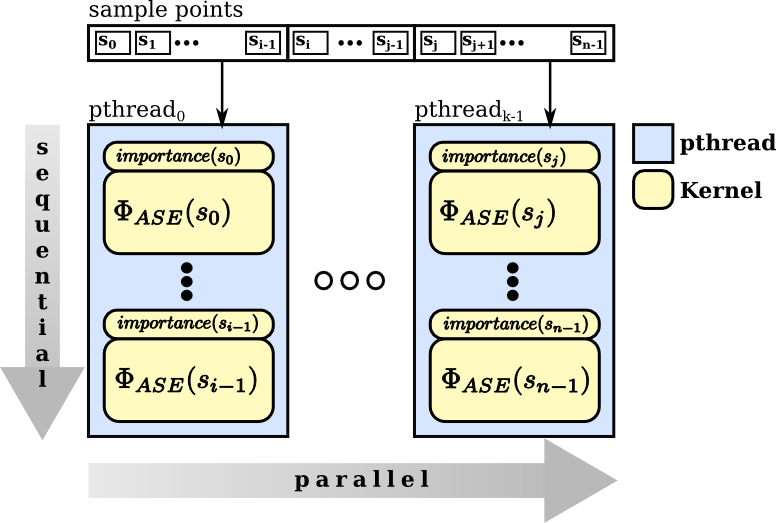
\includegraphics{graphics/multigpu_partitioning2.png}}}
  \caption{partitioning of the workload to multiple devices}
  \label{graphic:multigpu}
\end{figure}

\subsubsection{Rays as GPU threads}
\begin{figure}[H]
  \centerline
  {\resizebox{0.45\textwidth}{!}{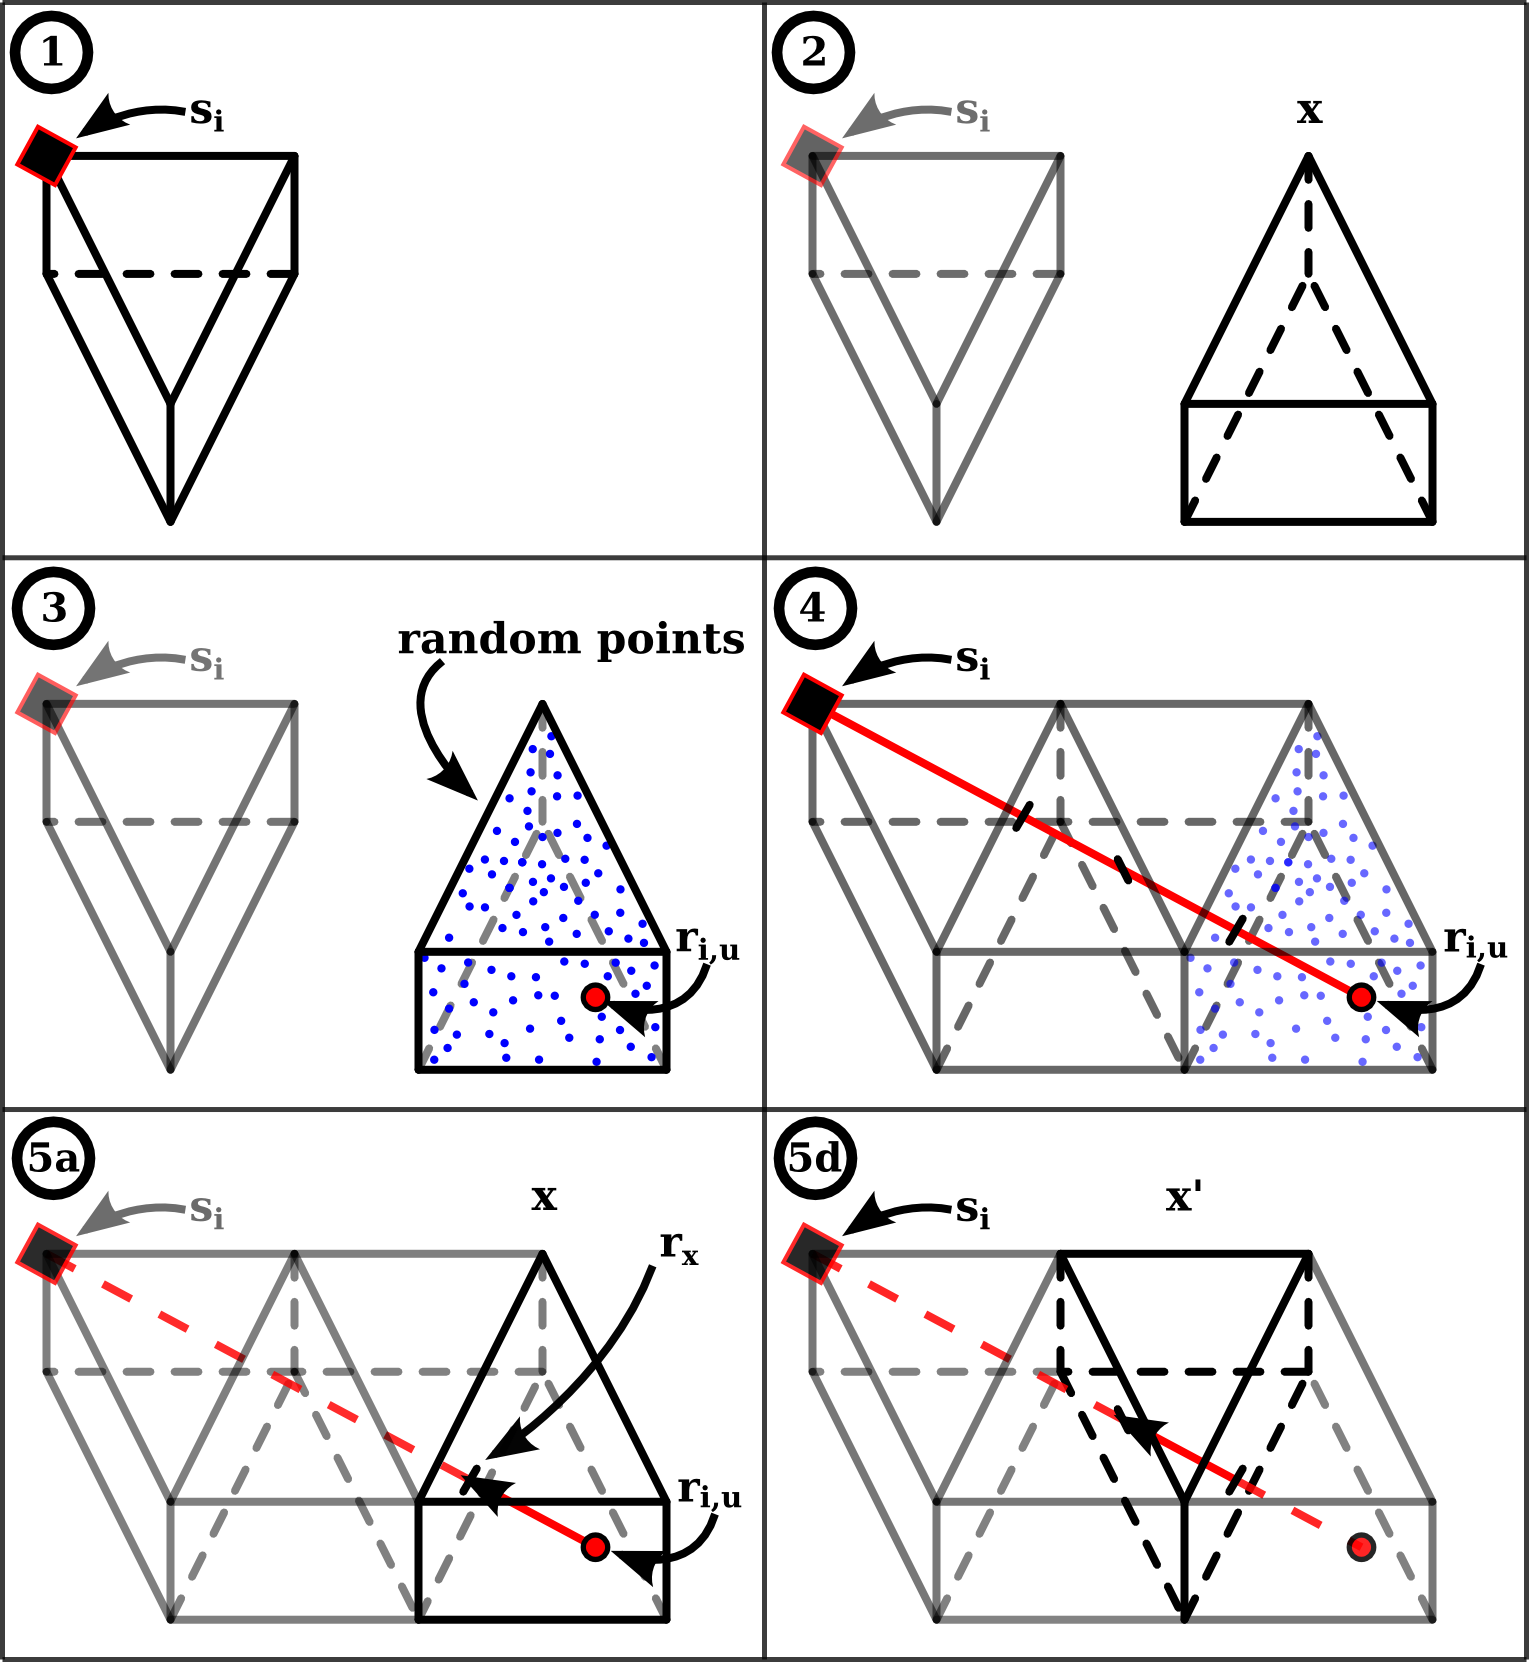
\includegraphics{graphics/iteration_detail4.png}}}
  \caption{steps for a single ray within a CUDA thread}
  \label{graphic:algorithm_steps}
\end{figure}
    The Raytracing of every ray can be done independently 
    through the mesh structure. 
    Exploiting this parallelism provides a great opportunity to boost
    performance. Figure \ref{graphic:kernel} demonstrates the distribution
    of rays to CUDA threads. In which a CUDA thread implements the following
    raytracing cycle:
    \begin{enumerate}
      \item Get current sample point $s_i$
      \item Request a prism to start ray from
      \item Generate start point $r_{i,u}$ inside this prism 
      \item Generate ray $\overrightarrow{r_{i,u}s_i}$
      \item Calculate $gain(\overrightarrow{r_{i,u}s_i})$ \eqref{eq:gain}
      \item Add gain to gain of the other rays atomically \eqref{eq:monte_carlo_ase}
    \end{enumerate}
    This repeats maximal $t$ times until every ray was traced. Furthermore rays with same
    origin and direction will be grouped into warps to utilize the
    GPU cache in a good way.
\begin{figure}[H]
  \centerline
  {\resizebox{0.5\textwidth}{!}{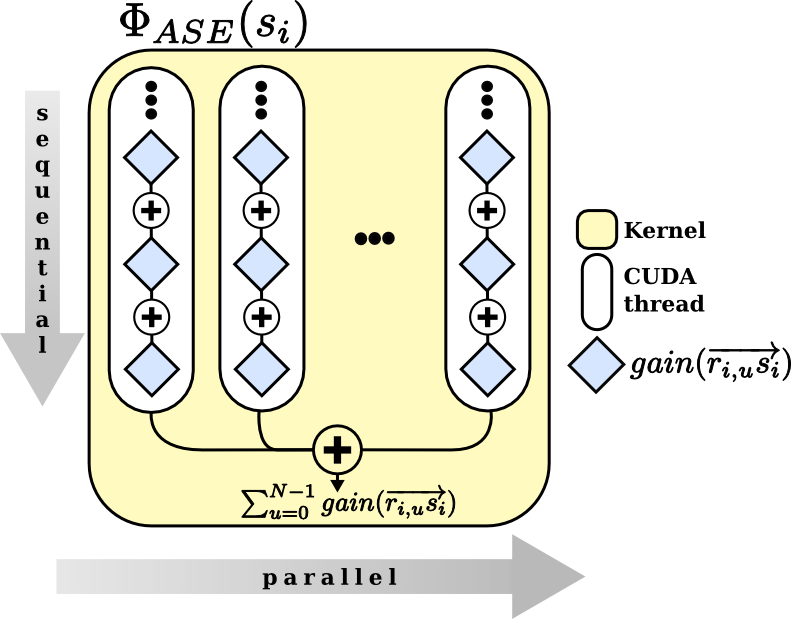
\includegraphics{graphics/kernel_detail3.png}}}
  \caption{$\Phi_{ASE}$ kernel with CUDA threads}
  \label{graphic:kernel}
\end{figure}
\begin{figure}[H]
  \centerline
  {\resizebox{0.35\textwidth}{!}{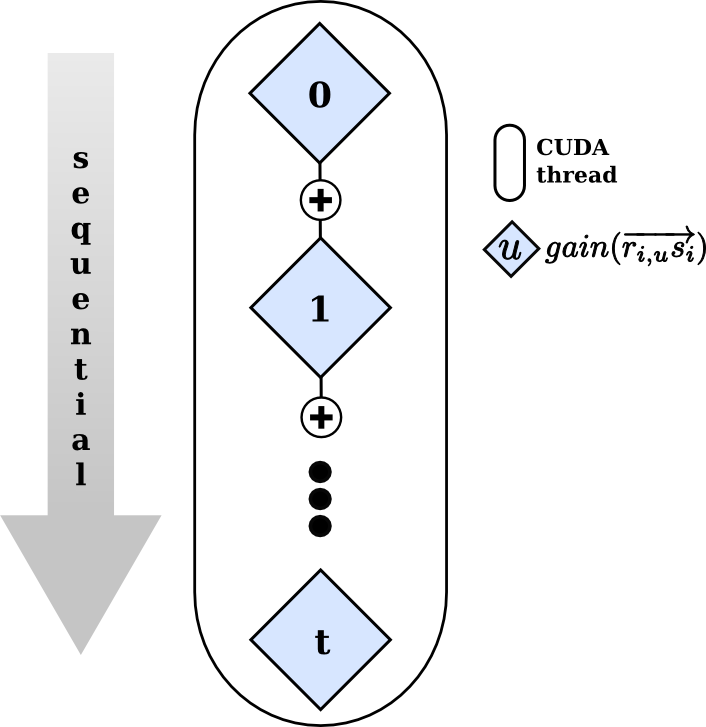
\includegraphics{graphics/thread_detail1.png}}}
  \caption{Multiple gain calculations within a single CUDA thread}
  \label{graphic:thread_detail}
\end{figure}

\subsection{Importance sampling}
\label{subsec:importance_sampling}
Importance sampling is a well known technique in the domain
of statistics \cite{importanceSamplingSource}. In case of 
ASE-Flux calculation, before every kernel call an importance sampling 
of a sample point is done to Figure out which areas are more
important to the result and thus need more rays then others.
This method has a strong impact on the precision of the simulation.

Figure \ref{graphic:importance} demonstrates
the differences between calculation with and without
importance sampling. It is shown each a cut through the active
gain medium in which the graphic without important
sampling has some peaks. To reduce peaks, the experiment
could be simulated with more rays, but this would increase
calculation time. Thus, importance sampling can increase the
efficiency of Monte Carlo simulations by reducing variance 
and simulation runtime. 
\begin{figure}[H]
  \centerline
  {\resizebox{0.45\textwidth}{!}{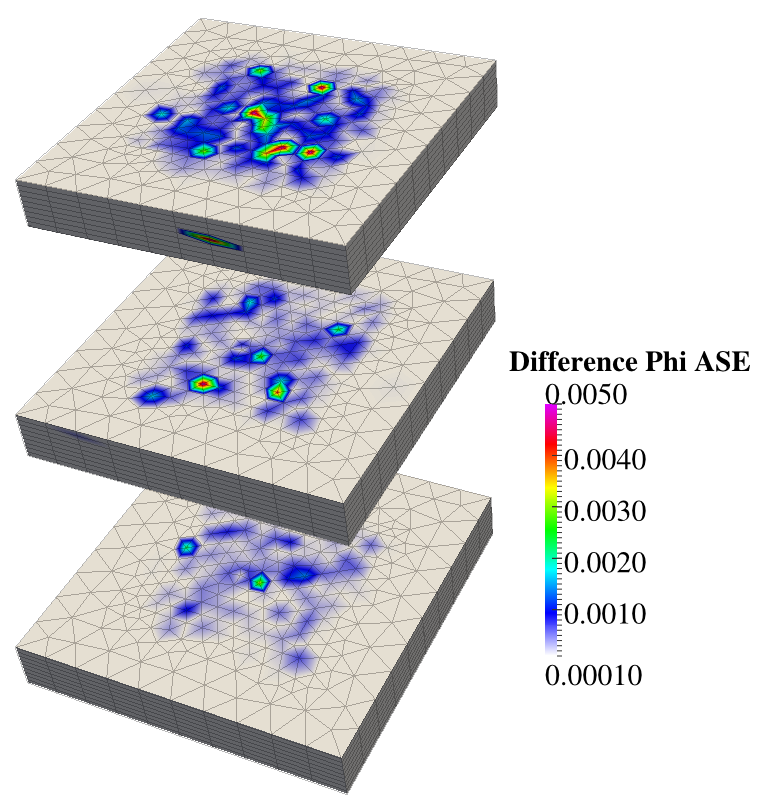
\includegraphics{graphics/phiASE_difference.png}}}
  \caption{Difference of $\Phi_{ASE}$ with and without importance sampling}
  \label{graphic:importance}
\end{figure}

\subsection{Adaptive sampling}
\label{subsec:adaptive_sampling}
Since most sample points behave in a good way, there is no need
to sample them with a high number of rays. Only some outliers need to
be sampled with a higher precision. To assess the precision
and therefore the difference between the true and calculated value,
it is further determined the mean squared error (MSE).
The adaptive method allows to remove strong peaks in the result
of the simulation without sampling all sample points with
a high number of rays resulting in reduced runtime.
%\end{multicols}
\begin{figure}[H]
  \centerline{
    \resizebox{0.5\textwidth}{!}{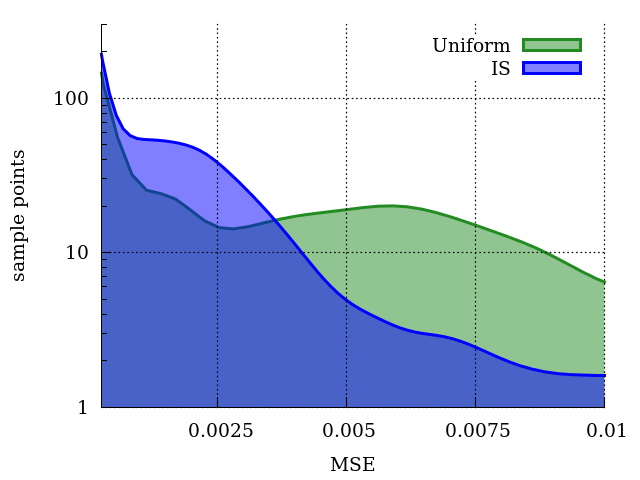
\includegraphics{plot/mse_importance.png}}}
  \caption{MSE histogram with and without importance sampling}
  \label{plot:adaptive}
\end{figure}
\begin{figure}[H]
  \centerline{
    \resizebox{0.5\textwidth}{!}{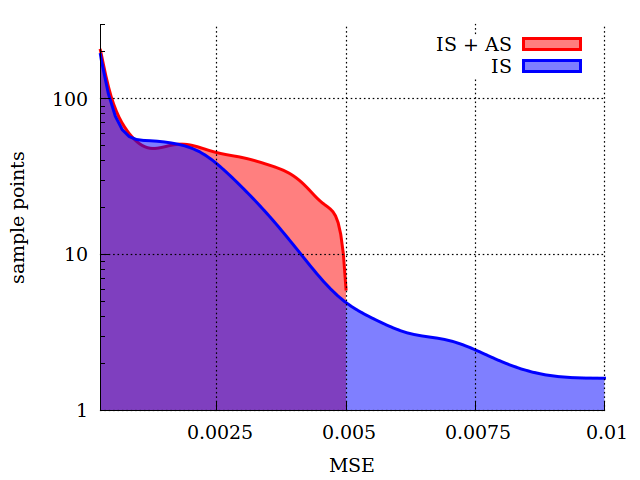
\includegraphics{plot/mse_adaptive.png}}}
  \caption{MSE histogram with and without adaptive sampling}
  \label{plot:adaptive2}
\end{figure}

%\begin{multicols}{2}

In Figure~\ref{plot:adaptive} the adaptive method with 
$5 \cdot 10^4$ to $5 \cdot 10^8$ rays per sample point is compared to the simulations
non adaptive and no importance sampling with each $3 \cdot 10^5$ rays per sample point (same runtime of 10s).
The not adaptive and no importance sampling method have some big peaks while all sample points of 
the adaptive method lie under a preset $MSE$-threshold (in this case 0.005). 

The adaptive method will not reduce the average MSE over sample points,
but it will reduce the maximal MSE values. Thus, using the adaptive
methods gives lower error by same calculation time.

%\begin{itemize}
%\item []
%     \[f(\vec{r_0}) = \frac{1}{n} \sum_{i=1}^n g_i \]
%     \[f^2(r_0) = \frac{1}{n} \sum_{i=1}^n g_i^2 \]
%     \[MSE(r_0) = \sqrt{\frac{f^2(r_0) - f(r_0)^2}{n}}\]
%\end{itemize}

